\chapter{適用例}\label{cha:Indication}
本章では、本研究で試作したツールが正しく動作することを、適用例を用いて確認する。
試作したツールに適用する帳票画像を、図\ref{fig:indication_original}に示す。
\begin{figure}[tp]
    \begin{center}
        \fbox{
            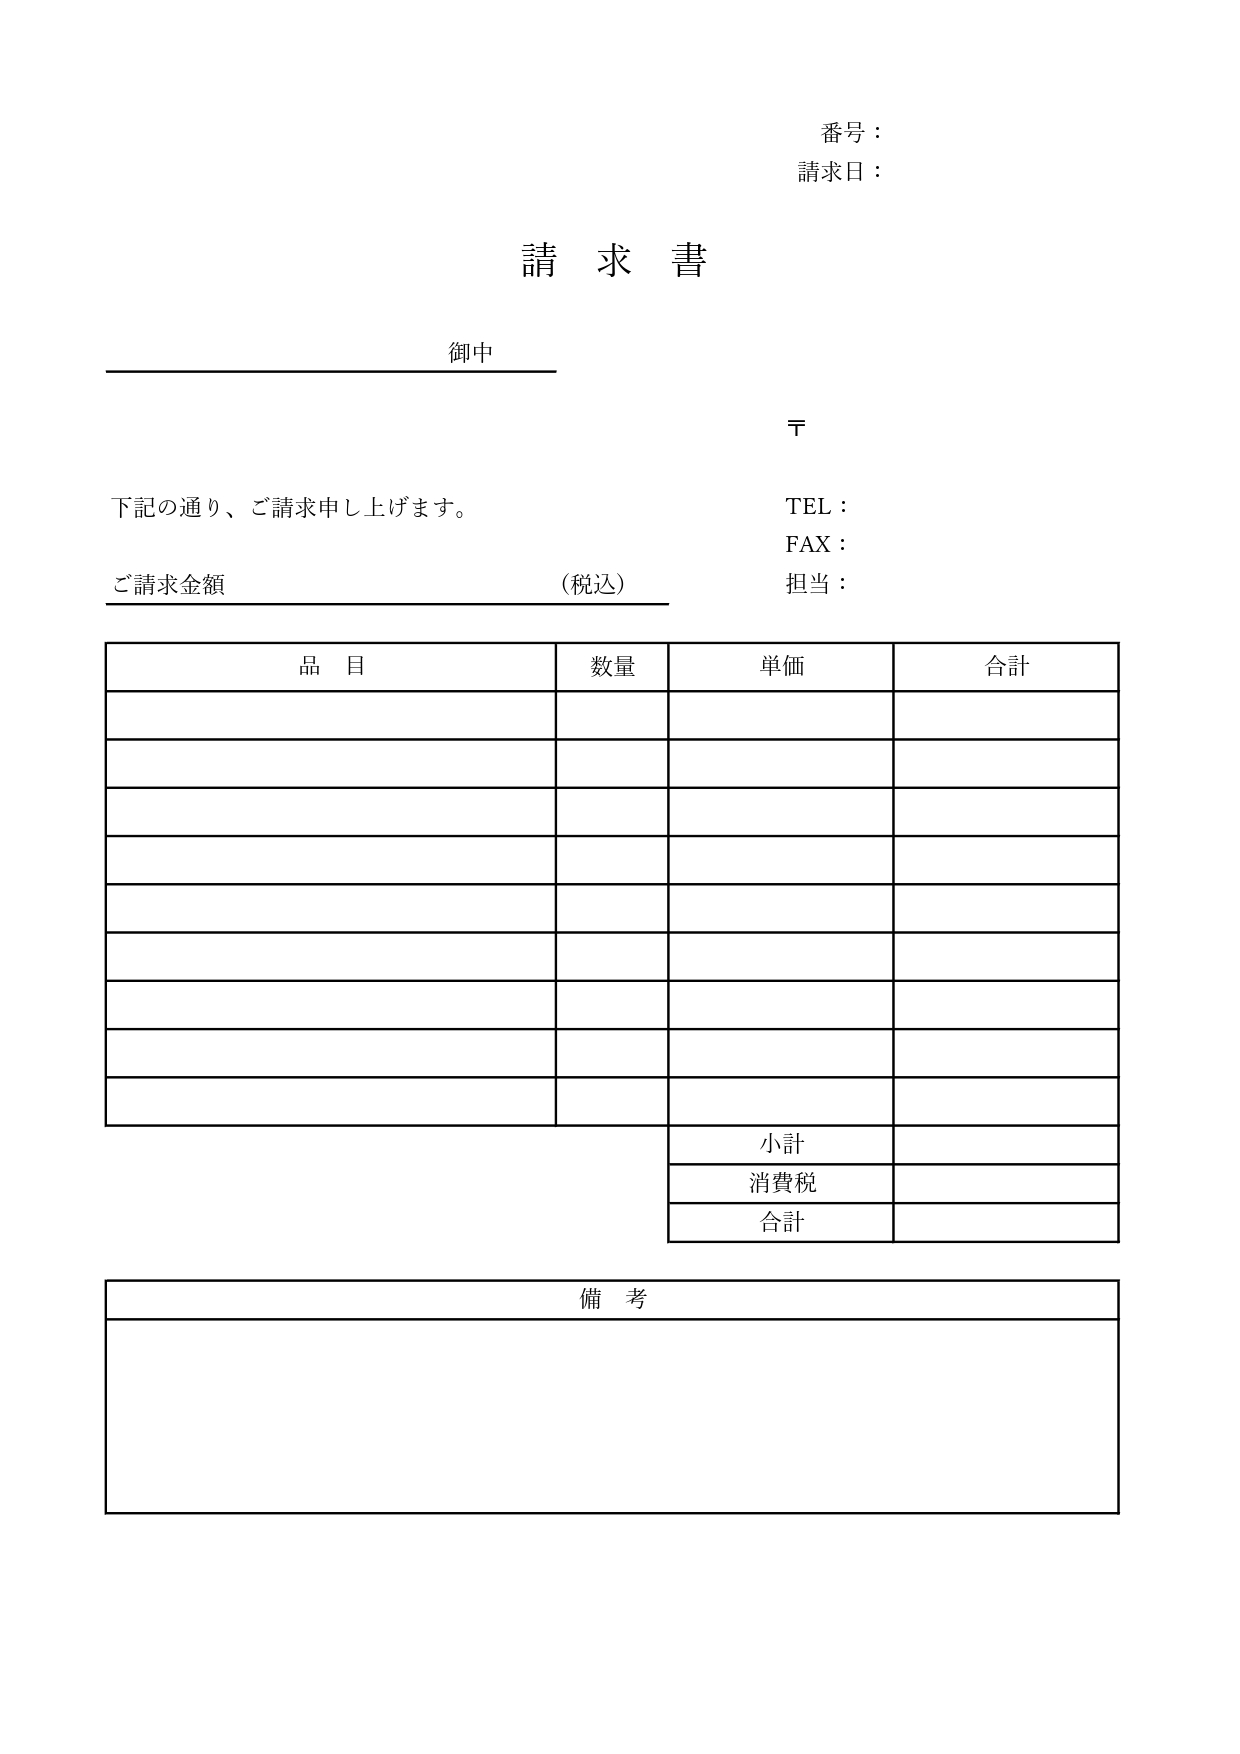
\includegraphics[width=15cm]{image/05-indication/indication_original.jpg}
        }
        \caption{試作したツールを適用する帳票画像}
        \label{fig:indication_original}
    \end{center}
\end{figure}

図\ref{fig:indication_original}に対して、試作したツールを適用し、出力であるJSONファイルと、矩形領域強調画像と下線部領域強調画像の2枚が、測定した矩形領域、下線部領域の位置、および、ラベルとそれぞれ一致することを確認する。
具体的には、JSONファイルのrects\_data配列と、矩形領域強調画像を参照し、矩形領域の出力結果を確認する。
同様に、JSONファイル内のunderlines\_data配列と、下線部領域強調画像を参照し、下線部領域の出力結果を確認する。

\section{矩形領域についての出力結果}\label{sec:result_rect}
本節は、矩形領域についての出力結果を確認する。

図\ref{fig:indication_original}に対して、試作したツールを適用し、出力したJSONファイルのうち、rects\_data配列の一部を、図\ref{fig:rects_data_json}に示す。
\lstset{language=}
\begin{figure}[tp]
    \begin{lstlisting}
        {
            "id": 4,
            "label": "string",
            "coords": {
                "top_left": {
                    "x": 275,
                    "y": 817
                },
                "buttom_left": {
                    "x": 275,
                    "y": 903
                },
                "buttom_right": {
                    "x": 1008,
                    "y": 903
                },
                "top_right": {
                    "x": 1008,
                    "y": 817
                }
            }
        },
        {
            "id": 5,
            "label": "number",
            "coords": {
                "top_left": {
                    "x": 1016,
                    "y": 817
                },
                "buttom_left": {
                    "x": 1016,
                    "y": 903
                },
                "buttom_right": {
                    "x": 1308,
                    "y": 903
                },
                "top_right": {
                    "x": 1308,
                    "y": 817
                }
            }
        },
    \end{lstlisting}
    \caption{rects\_data配列の一部}\label{fig:rects_data_json}
\end{figure}
また、図\ref{fig:rects_data_json}のJSONファイルと同時に出力した2枚の領域強調画像のうち、矩形領域を強調した画像の一部を、図\ref{fig:highlighted_rects_part}に示す。
\begin{figure}[tp]
    \begin{center}
        \fbox{
            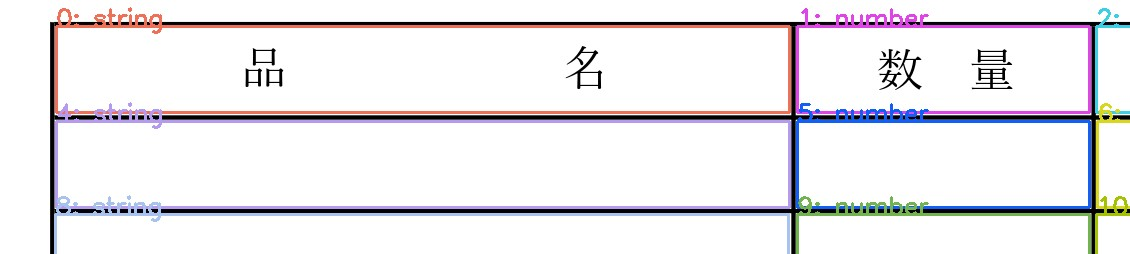
\includegraphics[width=15cm]{image/05-indication/highlighted_rects_part.jpg}
        }
        \caption{矩形領域を強調した画像の一部}
        \label{fig:highlighted_rects_part}
    \end{center}
\end{figure}

矩形領域座標について、IoU(Intersection over Union)を用いてJSONファイルの出力が正しいことを確認する。

測定したの矩形領域座標と、出力するJSONファイルの矩形領域座標を確認し、IoUを算出する。
図\ref{fig:rects_data_json}より、idキーの値が4である矩形領域座標は、左上頂点のxy座標が(275,817)であり、右下頂点のxy座標が(1008,903)である。
図\ref{fig:highlighted_rects_part}にある4番の矩形領域について、図\ref{fig:indication_original}の画像では、左上頂点のxy座標が(273,816)であり、右下頂点のxy座標が(1009,905)であった。
よって、IoUを算出すると、0.96となる。
IoUが閾値である0.5以上であるため、この矩形領域座標は正しく取得できたと言える。
他の矩形領域に対しても、矩形領域座標を正しく取得していることを確認した。

ラベルについて、人間が判断したラベルと、ツールが出力したラベルが一致するかを確認する。
図\ref{fig:rects_data_json}より、idキーの値が4と5である矩形領域について、それぞれラベルはstring、numberである。
図\ref{fig:highlighted_rects_part}より、画像内に描画した矩形領域の番号のうち、4番の矩形領域は「品名」を記入する欄であり、5番の矩形領域は「数量」を記入する欄であることがわかる。
各矩形領域のラベルについて、「品名」は文字列(string)、「数量」は数値(number)がそれぞれ正しいラベルであるため、これら2つの矩形領域について、正しいラベルを割り付けていることを確認できた。
他の矩形領域に対しても、一部を除き、正しいラベルを割り付けていることを確認した。

また、矩形領域について、JSONファイルと領域強調画像の出力が対応することから、帳票画像のレイアウトを保持したまま、矩形領域の領域座標とラベルを出力できたことがわかる。

一部の矩形領域については、本来割り付けるべきラベルとは異なるラベルを誤って割り付けた。
JSONファイルのうち、誤ったラベルを割り付けた矩形領域座標を、図\ref{fig:rects_data_miss_json}に示す。
\lstset{language=}
\begin{figure}[tp]
    \begin{lstlisting}
        {
            "id": 25,
            "label": "string",
            "coords": {
                "top_left": {
                    "x": 1713,
                    "y": 1283
                },
                "buttom_left": {
                    "x": 1713,
                    "y": 1369
                },
                "buttom_right": {
                    "x": 2262,
                    "y": 1369
                },
                "top_right": {
                    "x": 2262,
                    "y": 1283
                }
            }
        },
    \end{lstlisting}
    \caption{誤ったラベルを割り付けた矩形領域座標}\label{fig:rects_data_miss_json}
\end{figure}
また、図\ref{fig:rects_data_miss_json}に示した矩形領域座標に対応する矩形領域強調画像を、図\ref{fig:highlighted_rects_miss_part}に示す。
\begin{figure}[tp]
    \begin{center}
        \fbox{
            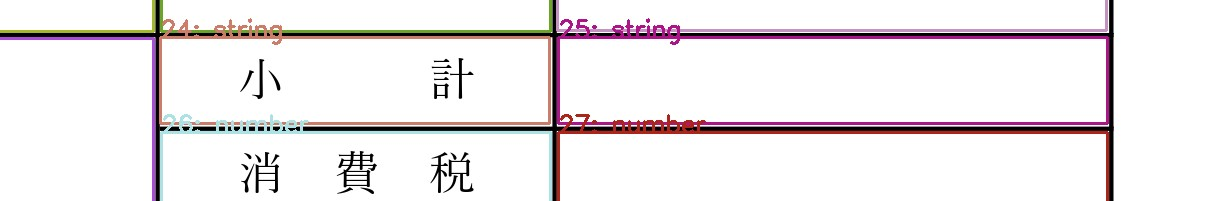
\includegraphics[width=15cm]{image/05-indication/highlighted_rects_miss_part.jpg}
        }
        \caption{図\ref{fig:rects_data_miss_json}の矩形領域を描画した矩形領域強調画像}
        \label{fig:highlighted_rects_miss_part}
    \end{center}
\end{figure}
図\ref{fig:rects_data_miss_json}より、idキーの値が25の矩形領域は、labelキーの値がstringであることがわかる。
図\ref{fig:highlighted_rects_miss_part}より、25番の矩形領域は、「小計」を記入する欄であることがわかる。
本来割り付けるべきラベルは数値(number)であるため、誤ったラベルを割り付けていることがわかる。
これは、「小計」という文字を認識することができなかったことが原因である。

図\ref{fig:indication_original}の画像に対して、認識した文字のバウンディングボックスを描画した画像の一部を、図\ref{fig:OCR_result}に示す。
\begin{figure}[tp]
    \begin{center}
        \fbox{
            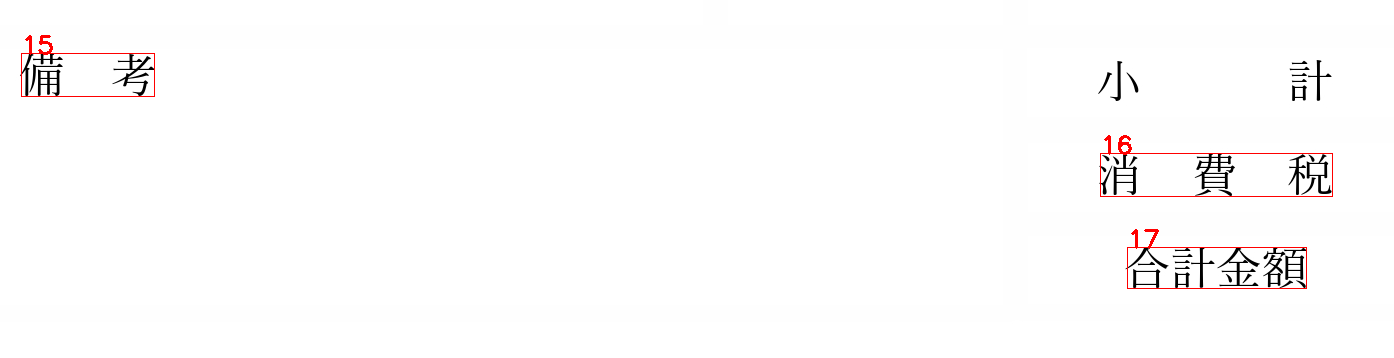
\includegraphics[width=15cm]{image/05-indication/OCR_result.png}
        }
        \caption{図\ref{fig:indication_original}で認識した文字}
        \label{fig:OCR_result}
    \end{center}
\end{figure}

図\ref{fig:OCR_result}の右にある「小計」については、バウンディングボックスを描画していないため、光学文字認識に失敗していることがわかる。
また、図\ref{fig:OCR_result}の左にある「備考」の文字について、属性を文字列(string)と推測したことを確認した。
このことから、光学文字認識を失敗したことによって、本来対応する文字とは別の文字の属性をラベルとして割り付けたことが、誤ったラベルを割り付けた原因であることがわかる。
この問題点については、\ref{sec:problems}節で後述する。

\section{下線部領域についての出力結果}\label{sec:result_underline}
本節は、下線部領域についての出力結果を確認する。

図\ref{fig:indication_original}に対して、試作したツールを適用し、出力したJSONファイルのうち、underlines\_data配列の一部を、図\ref{fig:underlines_data_json}に示す。
また、図\ref{fig:underlines_data_json}のJSONファイルと同時に出力した2枚の下線部強調画像のうち、下線部領域を強調した画像の一部を図\ref{fig:highlighted_underlines_part}に示す。
\lstset{language=}
\begin{figure}[tp]
    \begin{lstlisting}
        {
            "id": 0,
            "label": "date",
            "left": {
                "x": 869,
                "y": 354
            },
            "right": {
                "x": 1512,
                "y": 354
            }
        },
        {
            "id": 1,
            "label": "number",
            "left": {
                "x": 1908,
                "y": 355
            },
            "right": {
                "x": 2265,
                "y": 355
            }
        },
    \end{lstlisting}
    \caption{underlines\_data配列の一部}\label{fig:underlines_data_json}
\end{figure}
\begin{figure}[tp]
    \begin{center}
        \fbox{
            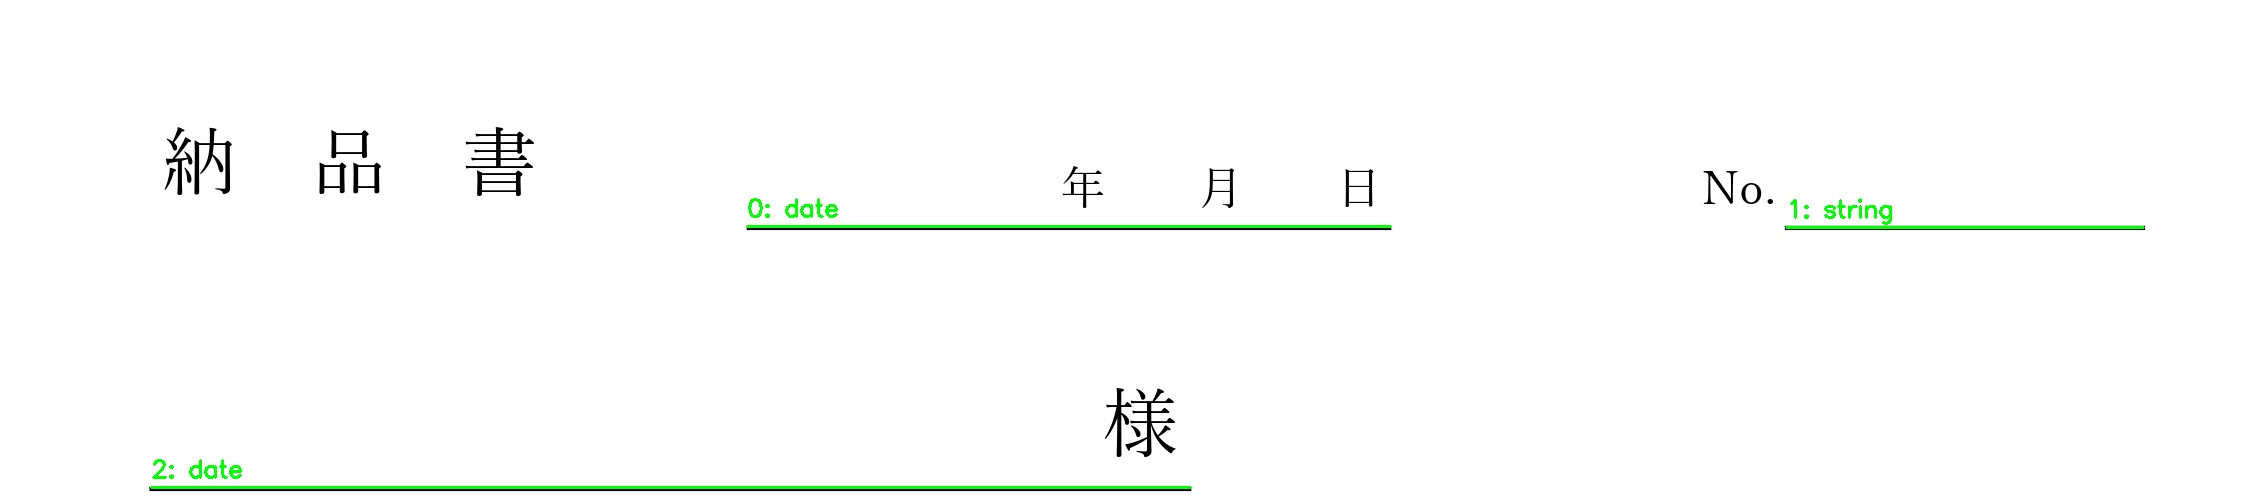
\includegraphics[width=15cm]{image/05-indication/highlighted_underlines_part.jpg}
        }
        \caption{下線部領域を強調した画像の一部}
        \label{fig:highlighted_underlines_part}
    \end{center}
\end{figure}
下線部領域座標について、矩形領域座標と同様に、IoUを用いてJSONファイルの出力が正しいことを確認する。
なお、下線部領域については、高さを3ピクセルとしてIoUを計算する。
測定した下線部領域座標と、出力するJSONファイルの下線部領域座標を確認し、IoUを算出する。
図\ref{fig:underlines_data_json}より、idキーの値が0である下線部領域座標は、左端点のxy座標が(869,354)であり、右端点のxy座標が(1512,354)である。
図\ref{fig:highlighted_underlines_part}にある0番の下線部領域について、図\ref{fig:indication_original}の画像では、左端点のxy座標が(869,354)であり、右端点のxy座標が(1511,354)であった。
よって、IoUを算出すると、0.99となる。
IoUが閾値である0.5以上であるため、この下線部領域座標は正しく取得できたと言える。
他の下線部領域に対しても、下線部領域座標を正しく取得していることを確認した。

下線部領域のラベルについて、人間が判断したラベルと、ツールが出力したラベルが一致するかを確認する。
図\ref{fig:underlines_data_json}より、idキーの値は0と1であり、それぞれラベルはdate、numberである。
図\ref{fig:highlighted_underlines_part}より、画像内に描画した矩形領域の番号のうち、0番の下線部領域は「年月日」を記入する欄であり、1番の下線部領域は番号である「No.」を記入する欄であることがわかる。
「年月日」は日付(date)、「No.」は数値(number)がそれぞれ正しいラベルであるため、これら2つの下線部領域について、正しいラベルを割り付けていることを確認できた。
他の下線部領域に対しても、一部を除き、正しいラベルを割り付けていることを確認した。

また、下線部領域について、JSONファイルと領域強調画像の出力が対応することから、帳票画像のレイアウトを保持したまま、下線部領域の領域座標とラベルを出力できたことがわかる。

一部の下線部領域については、本来割り付けるべきラベルとは異なるラベルを誤って割り付けた。
JSONファイルのうち、誤ったラベルを割り付けた下線部領域座標を、図\ref{fig:underlines_data_miss_json}に示す。

\lstset{language=}
\begin{figure}[tp]
    \begin{lstlisting}
        {
            "id": 2,
            "label": "date",
            "left": {
                "x": 273,
                "y": 615
            },
            "right": {
                "x": 1312,
                "y": 615
            }
        },
    \end{lstlisting}
    \caption{誤ってラベルを割り付けた下線部領域}\label{fig:underlines_data_miss_json}
\end{figure}

図\ref{fig:underlines_data_miss_json}の下線部領域は、図\ref{fig:highlighted_underlines_part}の2番の下線部領域である。
図\ref{fig:underlines_data_miss_json}より、idキーの値が2の下線部領域は、labelキーの値がdateであることがわかる。
図\ref{fig:highlighted_underlines_part}の左下を確認すると、2番の下線部領域は、右にある「様」という文字から、宛名を記入する欄であることがわかる。
本来割り付けるべきラベルは文字列(string)であるため、誤ったラベルを割り付けていることがわかる。
これは、\ref{subsec:label_link_processing}節で述べたラベルを割り付ける手法では、領域座標の右にある文字の属性を参照しないことが原因である。
この問題点については、\ref{sec:problems}節で後述する。